%\documentclass[preprint,3p,times,twocolumn]{elsarticleUS}
\documentclass[review,3p,times]{elsarticleUS}
\usepackage{amssymb}
\usepackage{amsmath}
\usepackage{graphicx}
\usepackage{bm}
\usepackage{yhmath}
\usepackage{subfigure}
\usepackage{multirow}
\usepackage{color}
\usepackage{xcolor}
\usepackage{subdepth}
\usepackage[nomarkers,lists]{endfloat}

\def\pp#1#2{\frac{\partial #1}{\partial #2}}

\biboptions{comma,sort&compress}

\journal{Combustion and Flame}

\makeatletter
\def\@author#1{\g@addto@macro\elsauthors{\normalsize%
    \def\baselinestretch{1}%
    \upshape\authorsep#1\unskip\textsuperscript{%
      \ifx\@fnmark\@empty\else\unskip\sep\@fnmark\let\sep=,\fi
      \ifx\@corref\@empty\else\unskip\sep\@corref\let\sep=,\fi
      }%
    \def\authorsep{\unskip,\space}%
    \global\let\@fnmark\@empty
    \global\let\@corref\@empty  %% Added
    \global\let\sep\@empty}%
    \@eadauthor={#1}
}
\makeatother

\begin{document}

\begin{frontmatter}

\title{NTC-affected stabilization of nonpremixed DME/air jet flames}

\author{Sili~Deng\corref{cor}}
\author{Peng~Zhao}
\author{Michael E.~Mueller}
\author{Chung K.~Law}
\cortext[cor]{Corresponding Author: silideng@princeton.edu}

\address{Department of Mechanical and Aerospace Engineering, Princeton University, Princeton, NJ 08544, USA}

\begin{abstract}
\textcolor{red}{TBD}

\end{abstract}

\begin{keyword} 
Negative Temperature Coefficient (NTC) \sep Dimethyl Ether (DME) \sep
Nonpremixed jets \sep Stabilization 
\end{keyword}

\end{frontmatter}

%\clearpage % For word count
\section{Introduction}

Nonpremixed jet flames have been extensively studied to understand the combustion processes in diesel engines.  The stabilization and structure of the jet flames determine the lifted height of the flame, therefore is crucial to the engine design.  Due to the mixing process of the fuel and oxidizer streams, the combustion mode is partially premixed, resulting in a two-dimensional tribracial flame~\cite{buckmaster02}, namely, a lean and a rich premixed flame wing with a trailing diffusion flame branch.  The point where the three branches intersect is called the triple point.  A recent review by Chung~\cite{chung07} discussed the stabilization, propagation and instability of tribrachial flames, including the the effects of concentration gradient, velocity gradient, and burnt gas expension.  Details about the referred experimental observations and computational simulations can be found in the literatures therein. These studies, however, limited to the nonautoignitive conditions, while the real diesel engine is operated at elevated pressures and temperatures, where autoignitions might be activated and interact with the tribracial flame. 

Chung and co-workers~\cite{choi09,choi10,choi12} conducted a series of experiments to investigate the autoignition characteristics of laminar C$_1$ to C$_4$ fuel jets in a heated coflow air jet and found that above certain coflow temperatures, lifted flames could be estabilished through autoignitions.  In these studies, both the tribrachial structure for most autoignited cases and a repetitive behavior of extinction and reignition at the critical condition near blowout were observed.  However, the role that autoignition plays in the stabilization mechanism, as well as its influences on the tribrachial flame is still less understood.  

Furthermore, diesel fuels have two-stage ignition processes, where the first stage ignition is governed by the low temperature chemistry, and the second stage ignition is dominated by the high temperature chemistry.  In both low and high temperature regimes, the ignition delay time decreases as the intial temperature increases.  However, in the intermediate temperature regime, the competition between the low and high temperature chemistry results in increased iginition delay time as the initial temperature increases.  Therefore, this nonmonotonic response of the ignition delay time to increasing initial temperature is the referred as negative temperature coefficient (NTC), which has been extensively studied in homogeneous system, as it is strongly associated with engine knock.  Recently, a series of both computational and experimental studies adopting the nonpremixed counterflow configuration by Law and co-workers~\cite{law12,zhao13,deng14} have demonstrated that with the existance of nonuniformities in the flow, species, and temperature fields, the ignition characteristics of the nonpremixed flames can be fundamentally affected by the NTC, especially at elevated pressures.   

Therefore, the NTC-affected stabilization of nonpremixed lifted flames can be potentially important, yet few literatures provide detailed analysis.  Krisman \emph{et al.}~\cite{krisman14} firstly conducted a numercial study of the dimethyl ether (DME)/air mixing layer at 40 atmospheres and a temperature range of 700 to 1500 $K$ and observed polybrachial structures in the heat release profiles.  The mixture fractions corresponding to the stabilization points defined based on the hydroxyl radical (OH) mass fraction and the the first stage autoignition kernels based on the methoxymethyl-peroxy radical (CH$_3$OCH$_2$O$_2$) were compared with the most reactive mixture fractiond computed from homogeneous autoignitions under the same intial conditions.  Transport budget analysis based on selected species were performed to differentiate deflagrations from autoignitions.

The previous study on the polybrachial structure is intriguing, showing the coupling of the autoigntion and flame propagation.  However, further investigation should be made to study the detailed chemical structure of the polybrachial flame.  For example, tools for computational diagnostics, especially for dominating reaction identifications, are needed.  On the other hand, even the autoignition stabilized flame has a two-dimensional structure. Consequently, a direct comparison to the homogeneous autoignition is unable to distinguish the mixture fraction stratification effects and the flame propagation effects along the mixture fraction iso-contour on the autoignition front.     

In the present study, nonpremixed coflowing DME/air jets are simulated at 30 atmospheres with the oxidizer stream heated to activate autoignitions.  Detailed reaction mechanisms for low and high temperature DME oxidation~\cite{curran98,fischer00,curran00,zhao08} have been developed and validated for burner stabilized flames~\cite{kaiser00}, nonpremixed counterflow flame ignition~\cite{zheng05}, laminar flame speeds~\cite{qin05}, and studies using rapid compression machines~\cite{mittal08}.  In particular, the present computation was conducted using a skeletal mechanism of $39$ species~\cite{bansal11} reduced from the detailed mechanism of Zhao \emph{et al.}~\cite{zhao08}.  With fixed jet velocities, only the oxidizer jet boundary temperature was varied to investigate the corresponding lifted flame morphology, chemical structure, and dominating reaction pathways.  The stabilization mechanism of the lifed flame, as well as the interactions between the autoigntion front and the propagating flame was analyzed based on computational explosive mode analysis (CEMA) and one-dimensional Lagrangian flamelet model, which will be introduced in detail in the next section. 


\section{Computational Methodology}
\subsection{Numerical method and flow field specification}

The nonpremixed DME/air jets were simulated as an axisymmetric fuel jet at $300$ K in a heated coflow of air, under the pressure of $30$ atmospheres.  The burner consists of a $0.8$ mm I.D. central nozzle, which is ten times the wall thickness, and the coflow O.D. varies from $0.3$ to $0.39$ mm, corresponding to different domain lengths, as summarized in Table~\ref{table:domain}.     \textcolor{red}{Inlet part, velocity and inlet length. Might consider using the same grid size for all the cases...}

The Navier-Stokes equation with low-Mach assumption, the conservation equations of mass, species, and energy are solved using NGA, which is a parallel code using Message Passing Interface (MPI).  Details about the numerical methods are available in Desjardins \emph{et al.}~\cite{desjardins08}, and only a brief summary is provided here.

The low-Mach Navier-Stokes equation is discretized spatially with a second order centered scheme on a staggered mesh.  The spatial discretization of all the species mass fractions, temperature and mixture fraction relies on the WENO3 \textcolor{red}{Ref?} scheme.  The iterative second order semi-implicit Crank-Nicolson scheme of Pierce and Moin~\cite{pierce01} is adopted to proceed the time integration.  At each time step, the chemical source terms for species and energy equations are evalucated independently from the transport terms using the CVODE \textcolor{red}{Ref?}.  The diffusivities for the species transport equations are computed based on the nonunity constant Lewis number formulation.  

\subsection{Chemical Explosive Mode Analysis}

The numerical diagnostic tool, Chemical Explosive Mode Analysis (CEMA) was developed by Lu \emph{et al.}~\cite{lu10} and was adopted in the present study to identify flame and ignition structure in complex flows.  Briefly, the eigenvalues of the Jacobian matrix of the chemical source term based on the local species concentrations and temperature is evaluated and determined as the chemical modes.  The largest positive eigenvalue, the chemical explosive mode, describes the rate of the system runaway.  The projection of a reaction on the explosive mode is defined as the explosion participation index, whose absolute value indicates how sensitive the explosive mode is to the reaction.  In the present study, species concentrations and temperatures were sampled at certain locations of interest from the NGA simulation and processed with CEMA.  Based on the explosive mode and participation index, species and reactions having the most influence on ignition and flame structure can be readily identified.

\subsection{Lagrangian Flamelet Model}

Even for the autoignitive cases, a direct comparison with the homogeneous autoignition, in terms of the ignition characteristics, is inappropriate, as in the homogeneous system, transport both along and parallel to the mixture fracture gradient is neglected.  Especially, for fuels with NTC chemistry, the dissipation along the mixture fraction gradient direction can significantly modify the ignition characteristics~\cite{law12,deng14}.      



















\section{Results and Discussion}
\subsection{Identification of the low-temperature, NTC, flame} \label{sec:4.1}

Validation results for the experimental system are shown in Fig.~\ref{fig:M}.  Specifically, when the PMT captures the photons corresponding to the characteristic wavelength of HCHO (peaks around $400$ nm), it outputs negative impulses to the oscilloscope, with the amplitudes of these impulses represent the light intensity.  Figure~\ref{fig:M} shows that such signal intensity drops after replacing either N$_2$-diluted DME with pure N$_2$ issued from the lower nozzle (at point a), or air with N$_2$ issued from the upper nozzle (at point c), hence demonstrating that the signal is due to the simultaneous presence of air and DME.  Since replacing air with the same flow rate of N$_2$ barely affects the temperature profile and the flow field, the signal difference between the air/DME and N$_2$/DME cases indicates the existence of NTC chemical activities.  It is noted that the signal from N$_2$/DME thermal pyrolysis is minimal in the present study, such that the difference in the chemically reactive and non-reactive cases can be completely attributed to the low-temperature oxidation chemistry.  


\begin{figure}[t]
  \centering
  \scriptsize
  \vspace{-0.1in}
  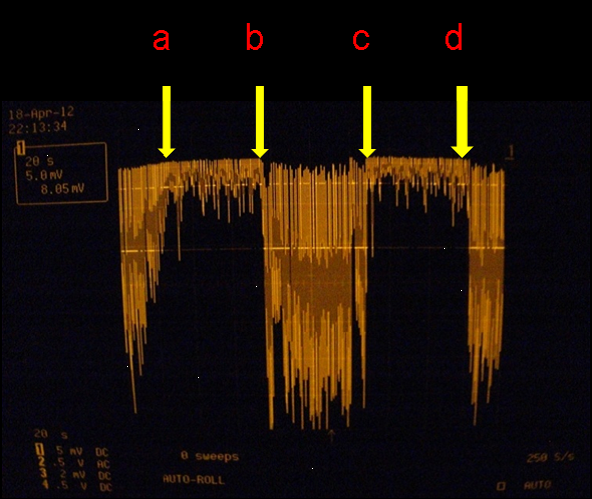
\includegraphics[width=0.5\textwidth]{M.png}
  \normalsize
%  \vspace{-0.1in}
  \caption{"M" shaped signal. a.~Switch Air/DME to Air/N$_2$; b.~Switch Air/N$_2$ to Air/DME; c.~Switch Air/DME to N$_2$/DME; d.~Switch N$_2$/DME to Air/DME.}
  \label{fig:M}
\end{figure}

In Fig.~\ref{fig:PMT}, the chemiluminescence intensity from the HCHO under the strain rates of $40$, $60$, and $100$ /s were measured as a function of the air boundary temperature.  The time-averaged signal were acquired by the lock-in amplifier with an integration time of three seconds to minimize the noise, and the error bars show the standard deviation of the signals based on $1000$ samplings. The results clearly show that the low-temperature chemistry becomes more pronounced at higher air temperatures and lower strain rates, with more HCHO produced and therefore stronger chemiluminescence from it.

\begin{figure}[t]
  \centering
  \scriptsize
  \vspace{-0.1in}
  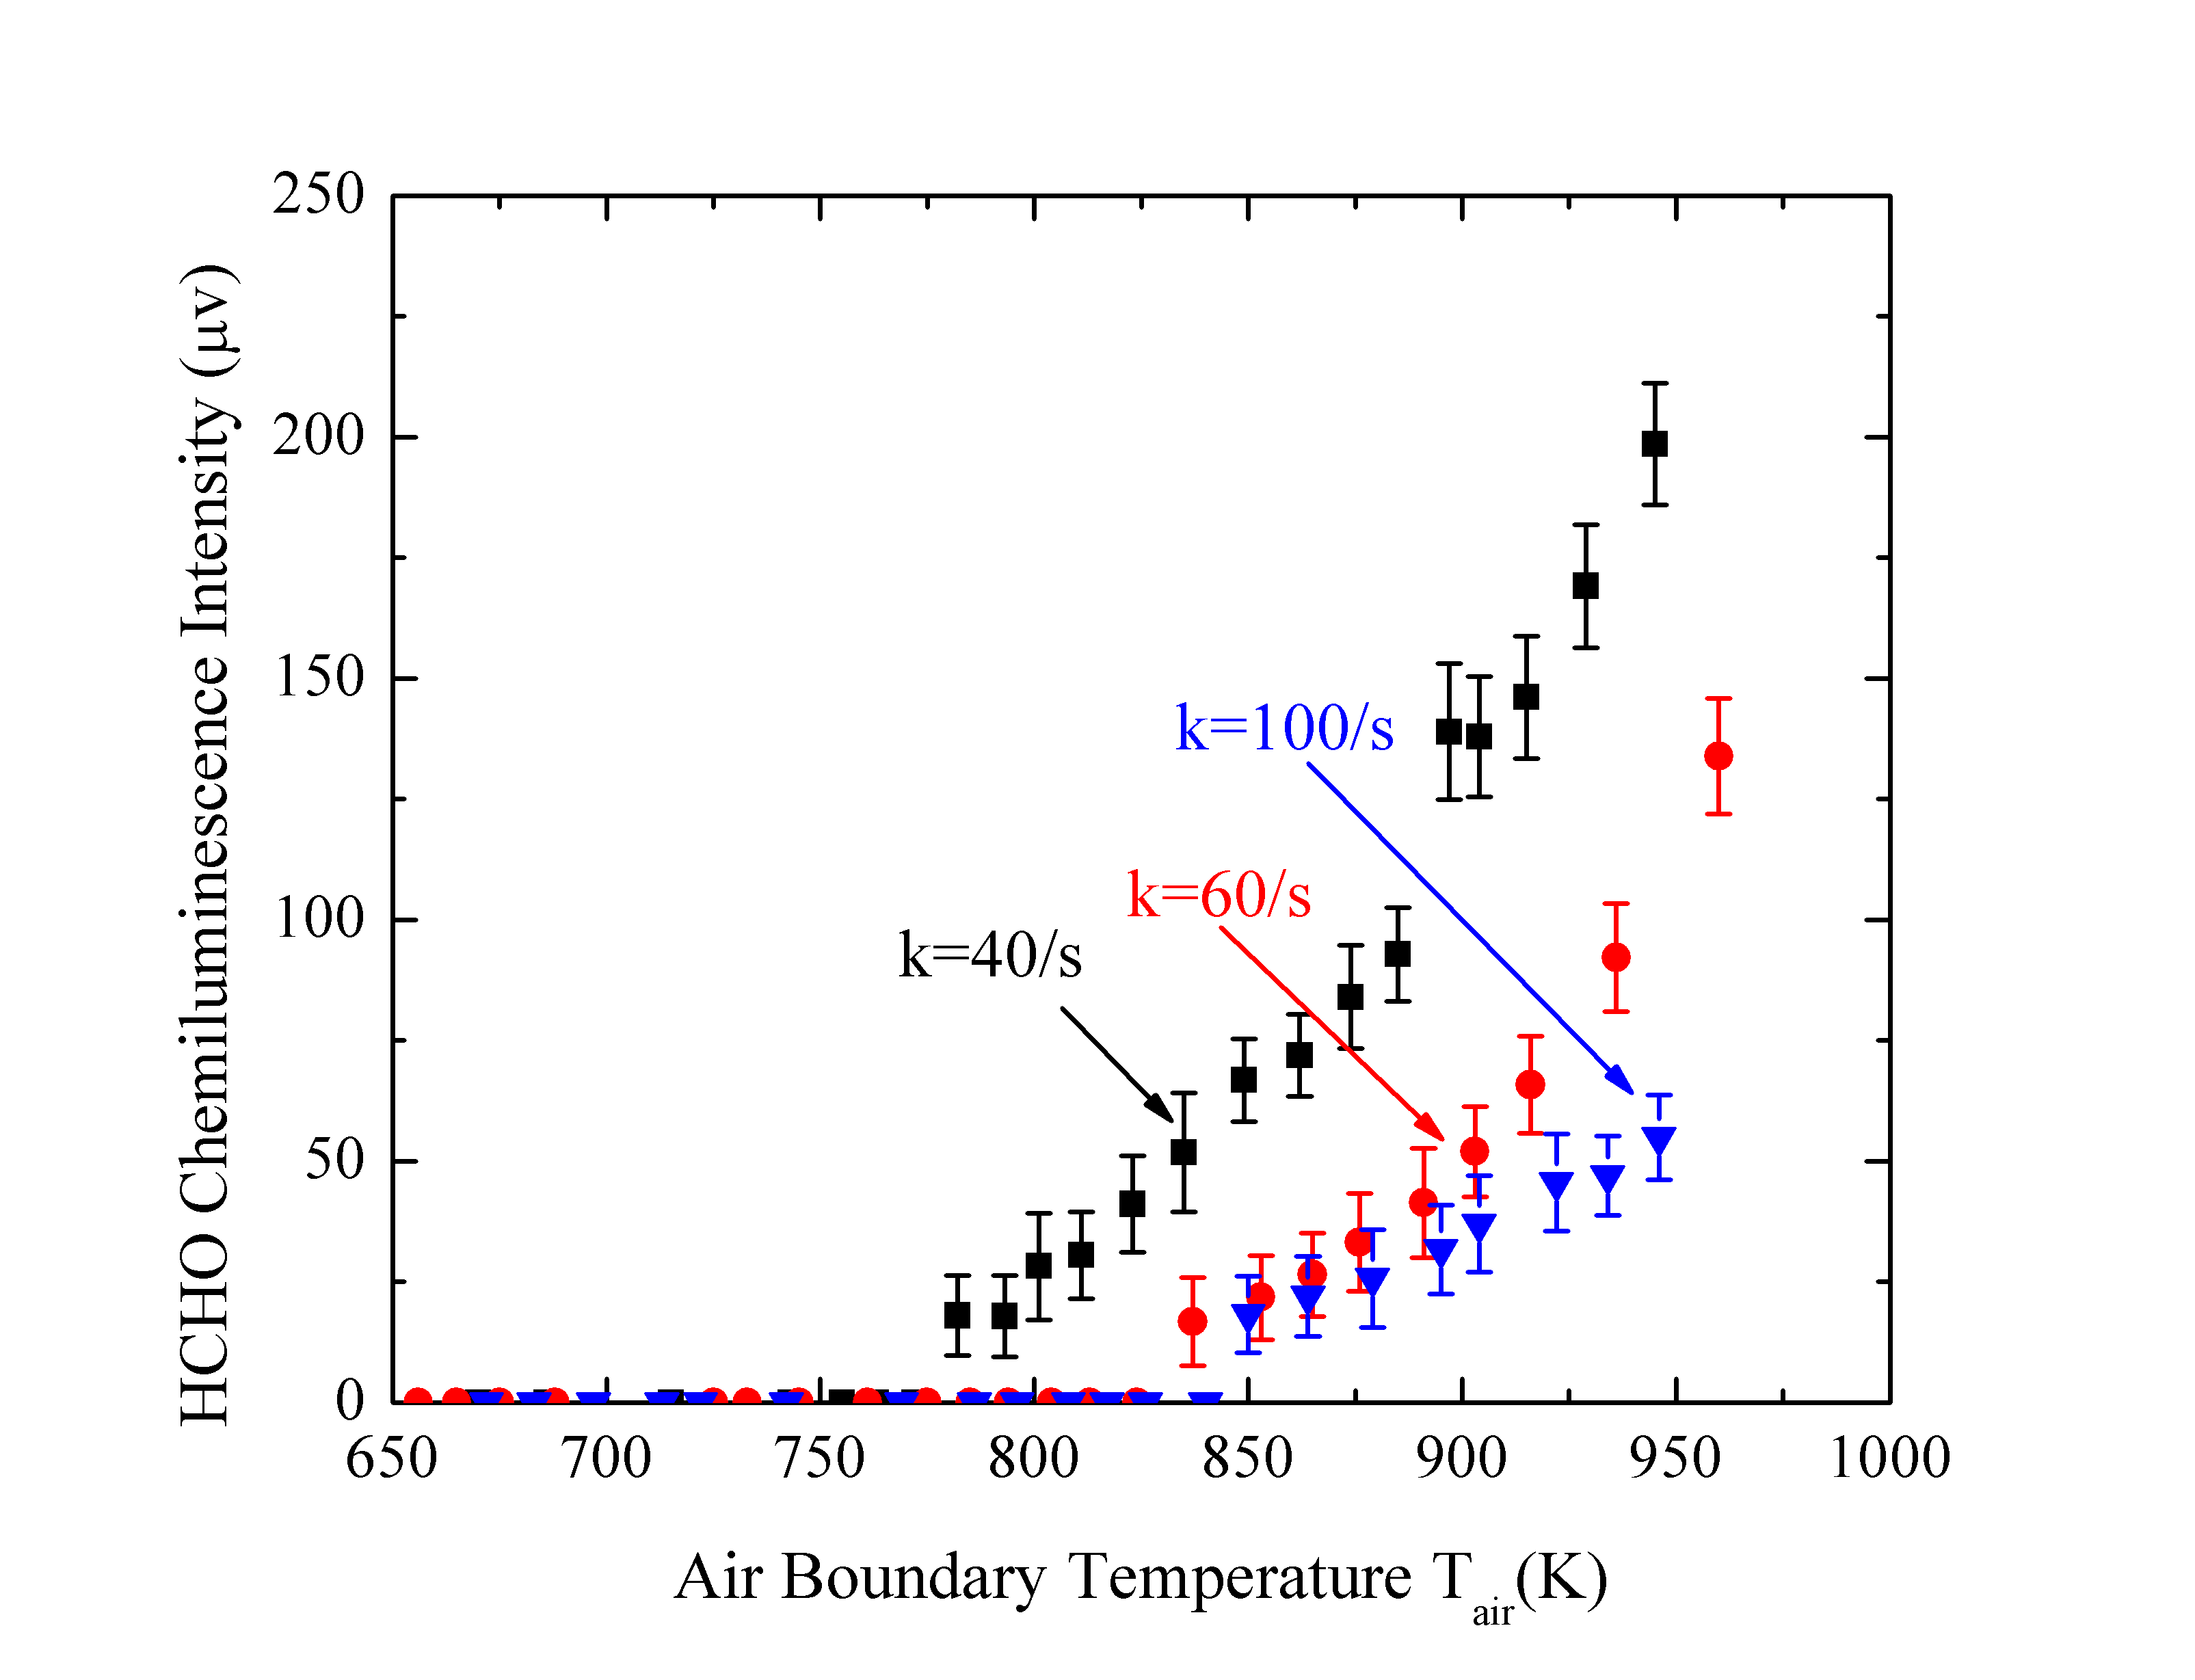
\includegraphics[width=0.6\textwidth]{PMT.png}
  \normalsize
  \vspace{-0.1in}
  \caption{HCHO chemiluminescence intensity at different air boundary temperatures under various strain rates.}
  \label{fig:PMT}
\end{figure}

The above experimental observations are further corroborated by the calculated results of the maximum formaldehyde (HCHO) mole fraction versus the air temperature for $30\%$ DME in nitrogen, for different strain rates.  Figure~\ref{fig:Scurve-SR} shows the calculated secondary S-curve characterized by the low-temperature chemistry.  It is seen that the upper branch solution, designating the state of the low-temperature flame, shows the same experimental trend of increasing HCHO concentration with increasing air temperature and decreasing strain rate.  We have therefore identified the presence of NTC-related chemical reactivity in the strongly transport-affected, nonpremixed counterflow.  The fact that this chemical reactivity is localized in a thin 鈥渇lame鈥?region is demonstrated in the next section.

\begin{figure}[t]
  \centering
  \scriptsize
  \vspace{-0.1in}
  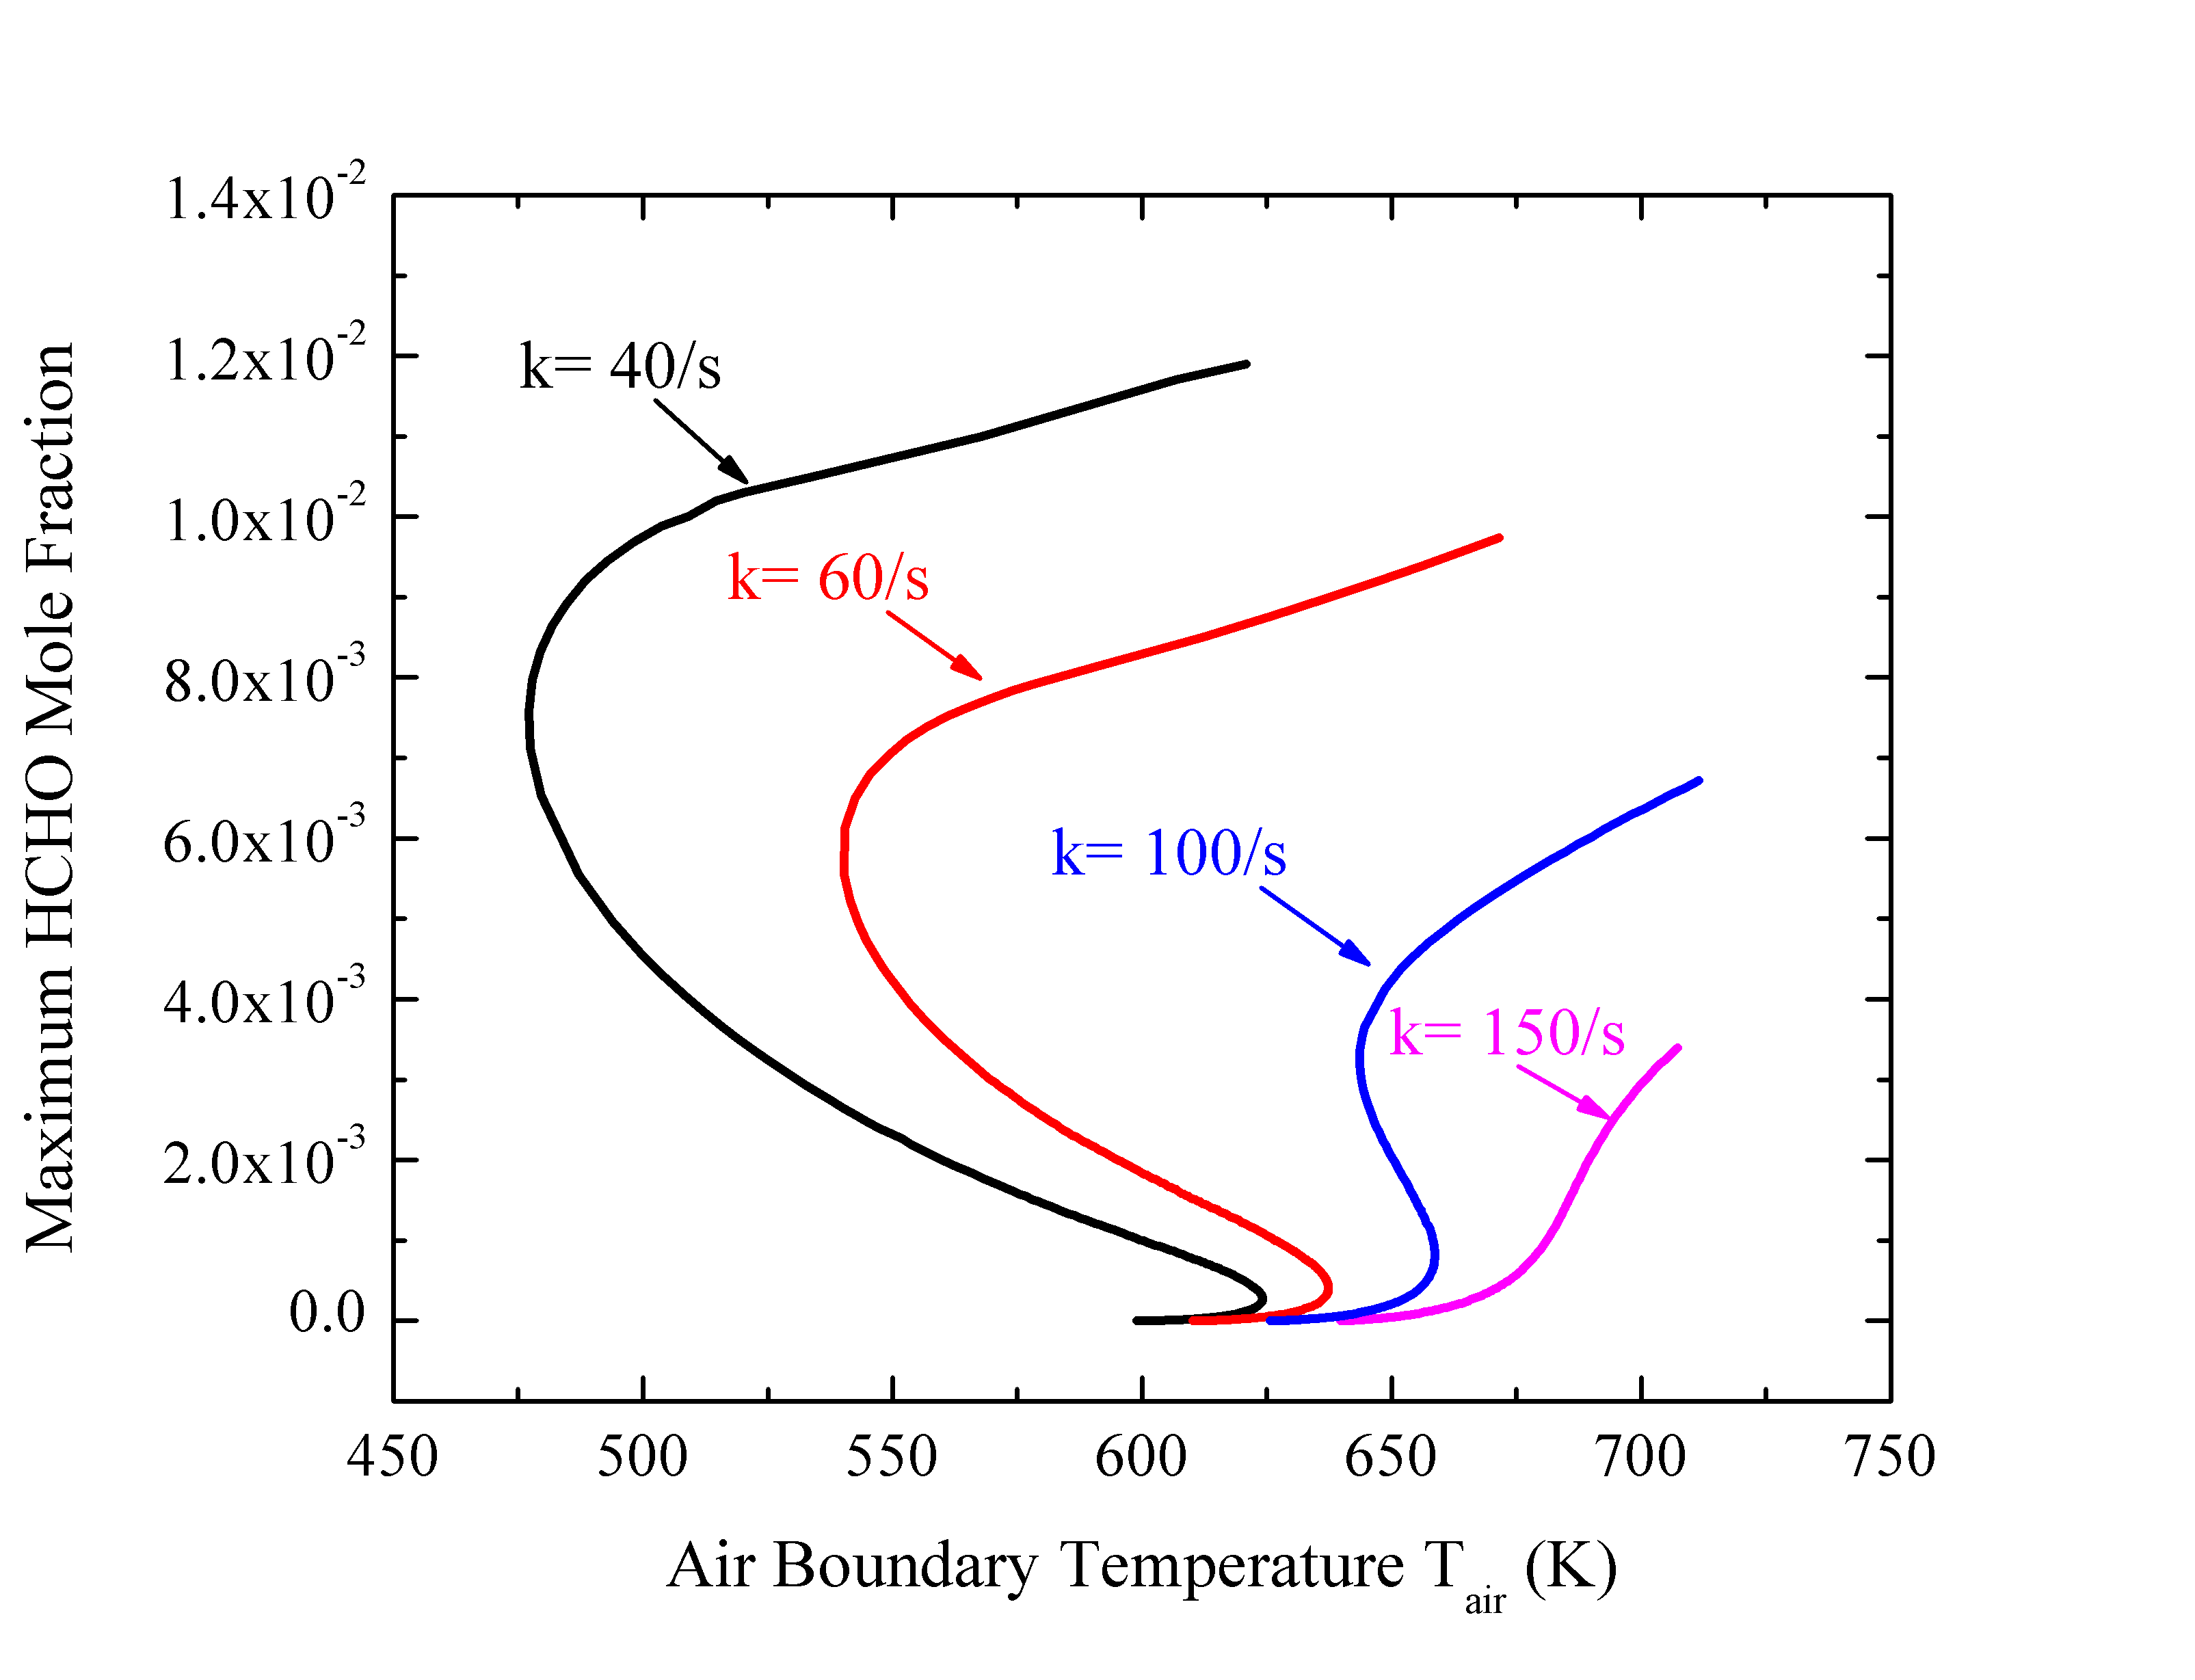
\includegraphics[width=0.6\textwidth]{Scurve-SR.png}
  \normalsize
  \vspace{-0.1in}
  \caption{Maximum HCHO mole fraction of $30\%$ DME at different air boundary temperatures under various strain rates.}
  \label{fig:Scurve-SR}
\end{figure}

\subsection{Determination of ignition temperature} \label{sec:4.2}

\begin{figure}[ht]
  \centering
  \scriptsize
  \vspace{0.1in}
  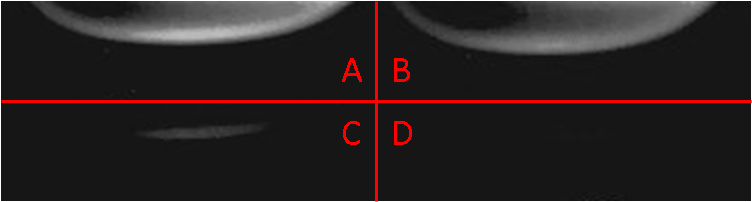
\includegraphics[width=0.5\textwidth]{IR.png}
  \normalsize
%  \vspace{-0.1in}
  \caption{A/B: Heated air/N$_2$ against DME counterflow IR images at ignition (atmospheric pressure, strain rate $60$ /s); C/D: Difference between A/B and B.}
  \label{fig:IR}
\end{figure}

We now proceed to detect the state of ignition of the NTC-flame, as identified by the lower turning points in Fig.~\ref{fig:Scurve-SR}.  Since the chemiluminescence intensity from the above experimentation is not strong enough to detect the low level of HCHO concentration at ignition, we have resorted to capturing the infrared radiation from the ignition process by using a highly sensitive infrared camera, FLIR SC640 (with the thermal sensitivity about $60$ mK at $303$ K), as shown on the right part of Fig.~\ref{fig:setup}.  The brightness of the IR images in Fig.~\ref{fig:IR} indicates the IR radiation intensity, with the bright color denoting higher radiation intensity than the dark color.  Since both the air/DME and N$_2$/DME flows now radiate infrared signals when heated due to the excitation of the vibrational modes of the gas molecules in the thermal mixing layer, the 鈥渂ackground鈥?N$_2$/DME signal needs to be subtracted out from the air/DME signal so as to isolate/identify the emission due to the low-temperature chemical reactivity.  Consequently, by gradually increasing the air boundary temperature, and by setting the IR radiation intensity of the N$_2$/DME flow as the reference state, the first appearance of an excess signal from the air/DME flow would indicate the onset of ignition.  In practice, when the air boundary temperature reaches the regime of interests, only $1$ K is increased each time at the air boundary before the flow becomes steady again.  It is fairly clear that at a certain temperature, which is defined as the ignition point, the signal from air/DME starts to exceed that of the reference state.  Such temperature measurements are repeatable within $\pm 2$ K.  A typical result is shown in Fig.~\ref{fig:IR}, in which the A and B panels are the raw IR signals for heated air and N$_2$ against DME, which are respectively reactive and nonreactive.  Panels C and D respectively show the residue signals of panels A and B after the background signal from panel B is subtracted; the null signal for D is obtained by default.  The temperature at which a discernable image of radiation is detected is then identified as that of ignition, as is the case for panels A/C, for the corresponding strain rate.

The localized nature of the IR radiation, shown in panel C, then also supports the notion that the chemical reactivity observed herein has the characteristic of a flame, in support of the interpretation of the chemiluminescence signal reported in the previous section.

Figure~\ref{fig:Ign-SR} shows the IR measurements of the low-temperature chemistry induced ignition, as determined through the above procedure, as a function of the strain rate.  The uncertainty bars account for those from the thermocouple radiation correction as well as reproducibility of the experimental measurements.  Due to the moderate flow field temperatures and the high sensitivity of the thermocouple, the uncertainty bars of the ignition temperatures are quite small.  These experimental values are then compared with those corresponding to the calculated lower, ignition turning points.  Figure~\ref{fig:Ign-SR} shows satisfactory agreement, with the average temperature difference being within $20$ K.

Sensitivity analysis was further performed for the state of ignition, as shown in Fig.~\ref{fig:Sen_SR}.  It is seen that the controlling chemistry is indeed the low tempearature chemistry, corresponding to the first stage ignition of the homogeneous autoignition process in the NTC-affect regime.  More specifically, the first two most important reactions that promote the low temperature chemistry induced ignition are the oxygen combination reaction: CH$_2$OCH$_2$O$_2$H+O$_2$ $\Leftrightarrow$ O$_2$CH$_2$OCH$_2$O$_2$H and the isomerization reaction: CH$_3$OCH$_2$O$_2$ $\Leftrightarrow$ CH$_2$OCH$_2$O$_2$H, while the most important retarding reaction is the $\beta$-scission reaction: CH$_2$OCH$_2$O$_2$H $\Leftrightarrow$ OH+$2$HCHO.  These two groups of reactions compete for the CH$_2$OCH$_2$O$_2$H radicals and as such function oppositely.

\begin{figure}[t]
  \centering
  \scriptsize
  \vspace{-0.1in}
  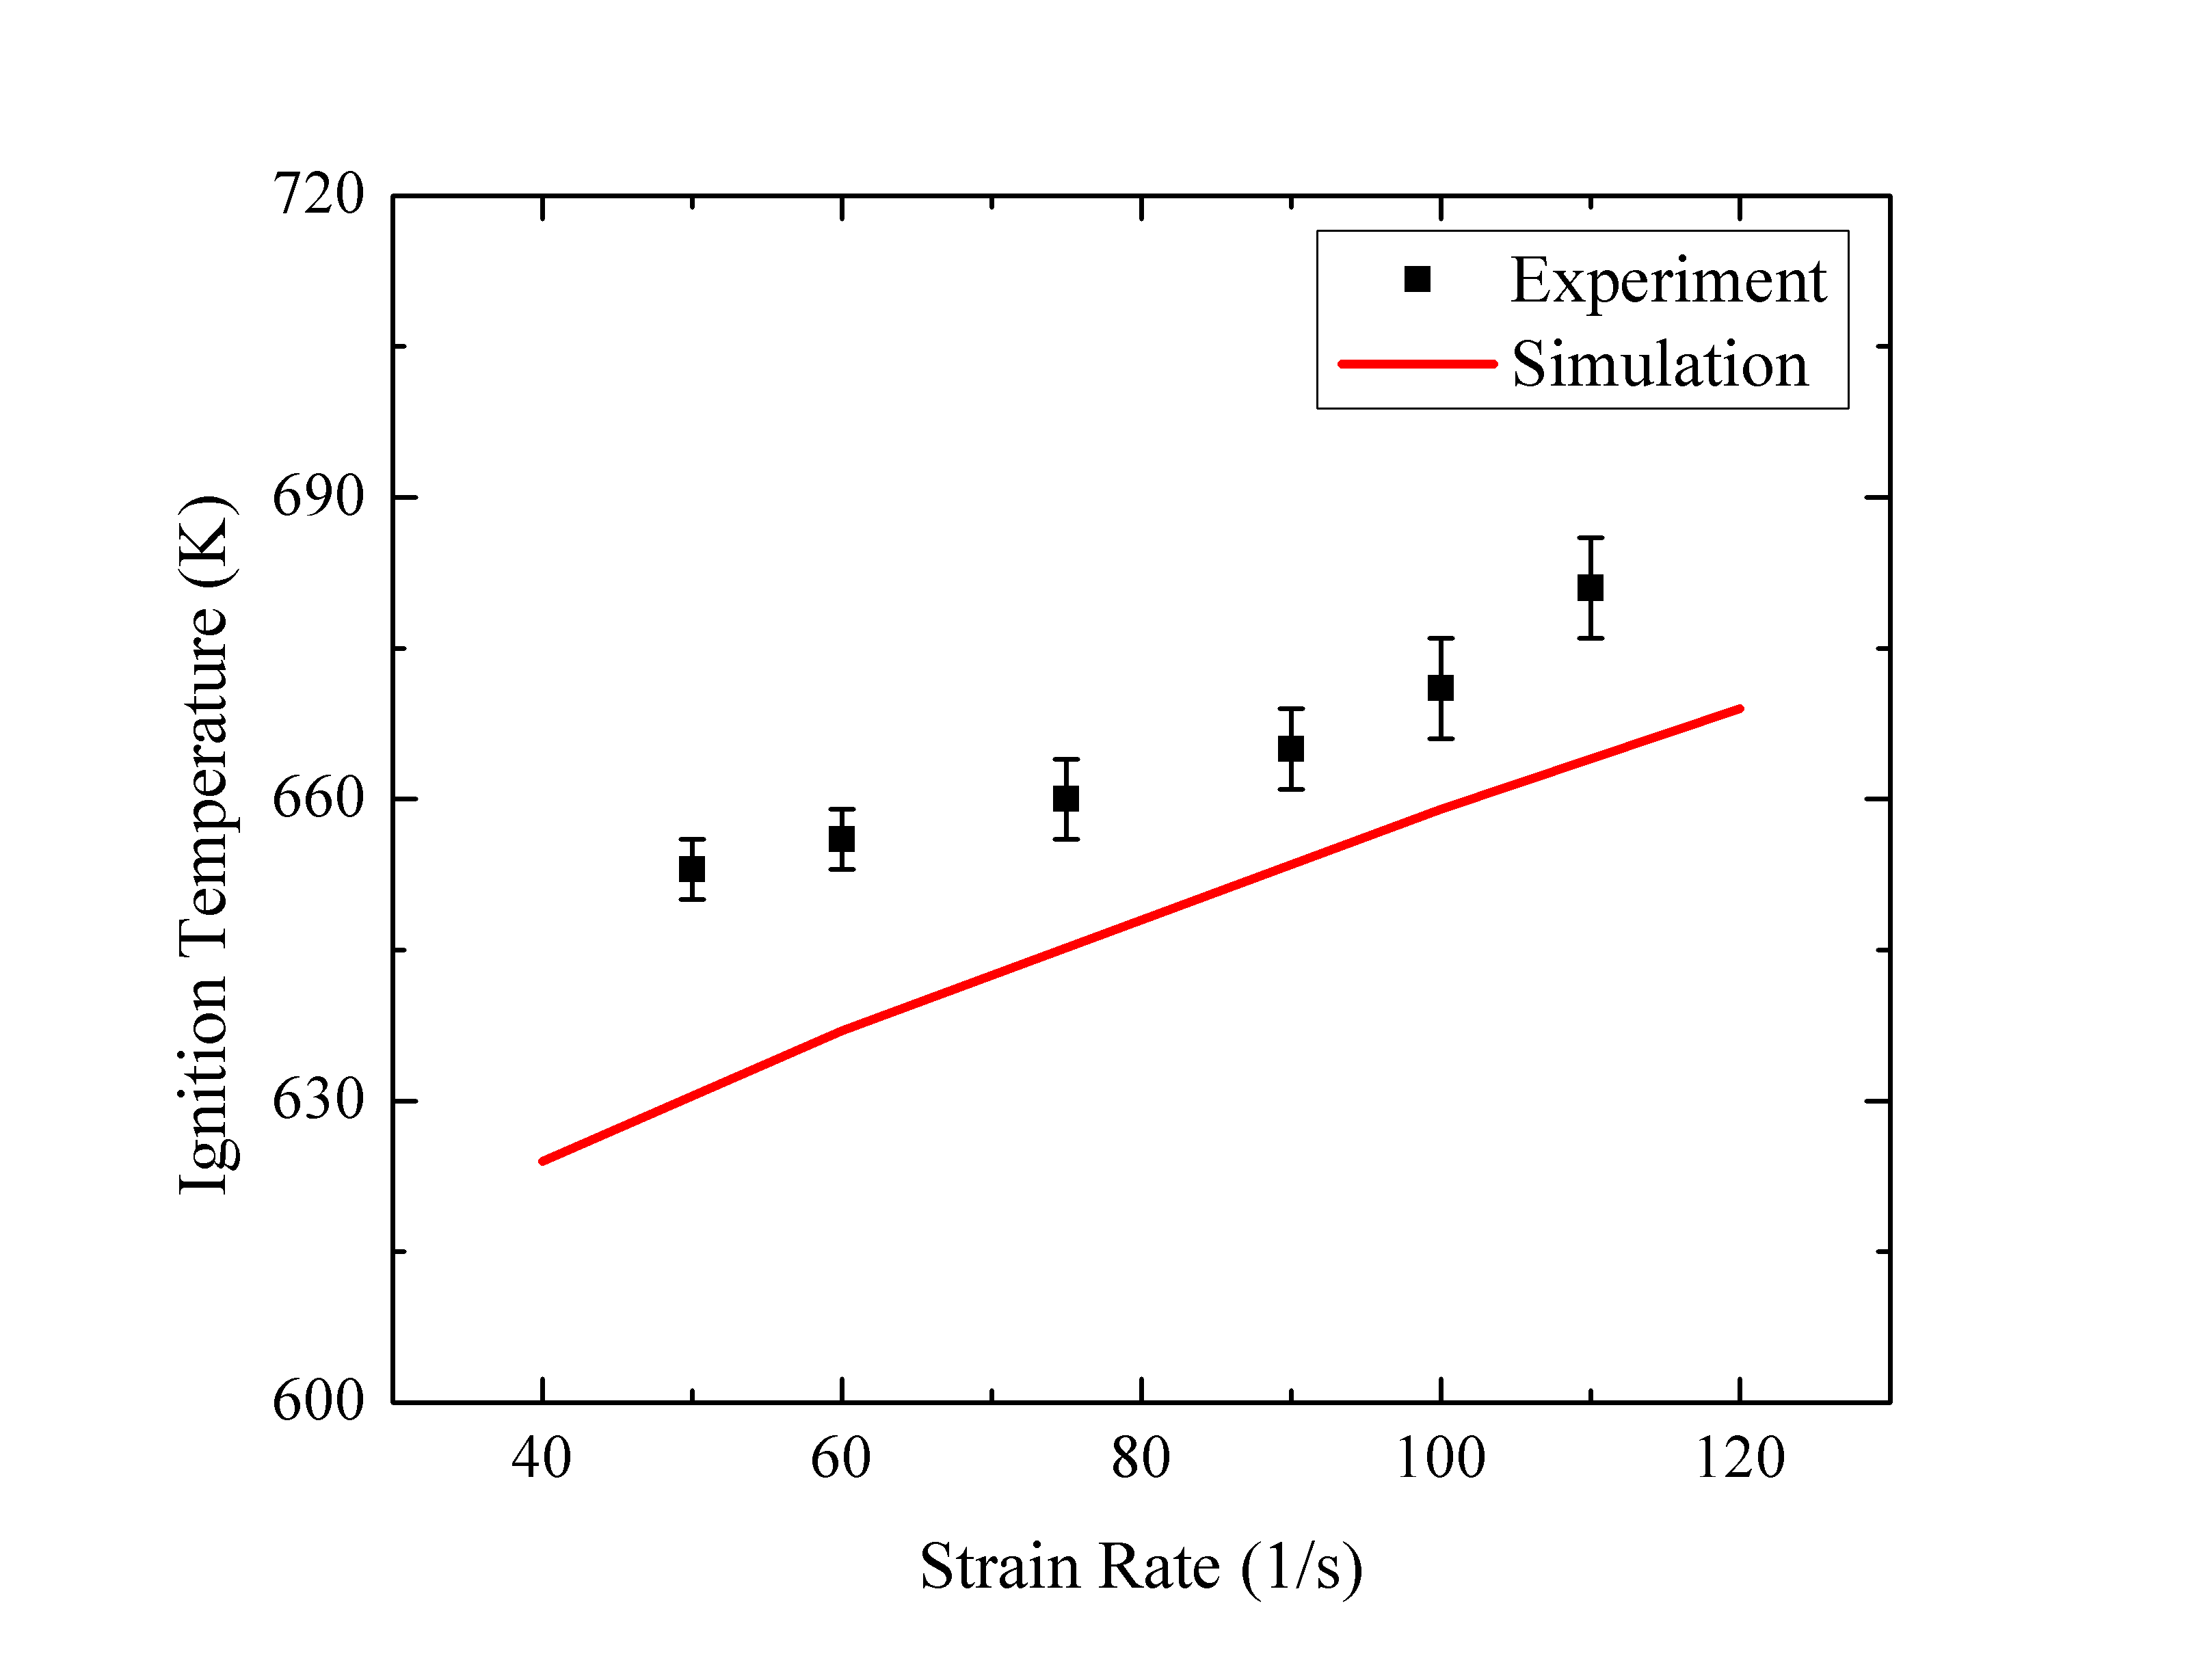
\includegraphics[width=0.6\textwidth]{Ign-SR.png}
  \normalsize
  \vspace{-0.1in}
  \caption{Calculated and observed ignition temperatures of $30\%$ DME under various strain rates.}
  \label{fig:Ign-SR}
\end{figure} 

\begin{figure}[t]
  \centering
  \scriptsize
  \vspace{-0.1in}
  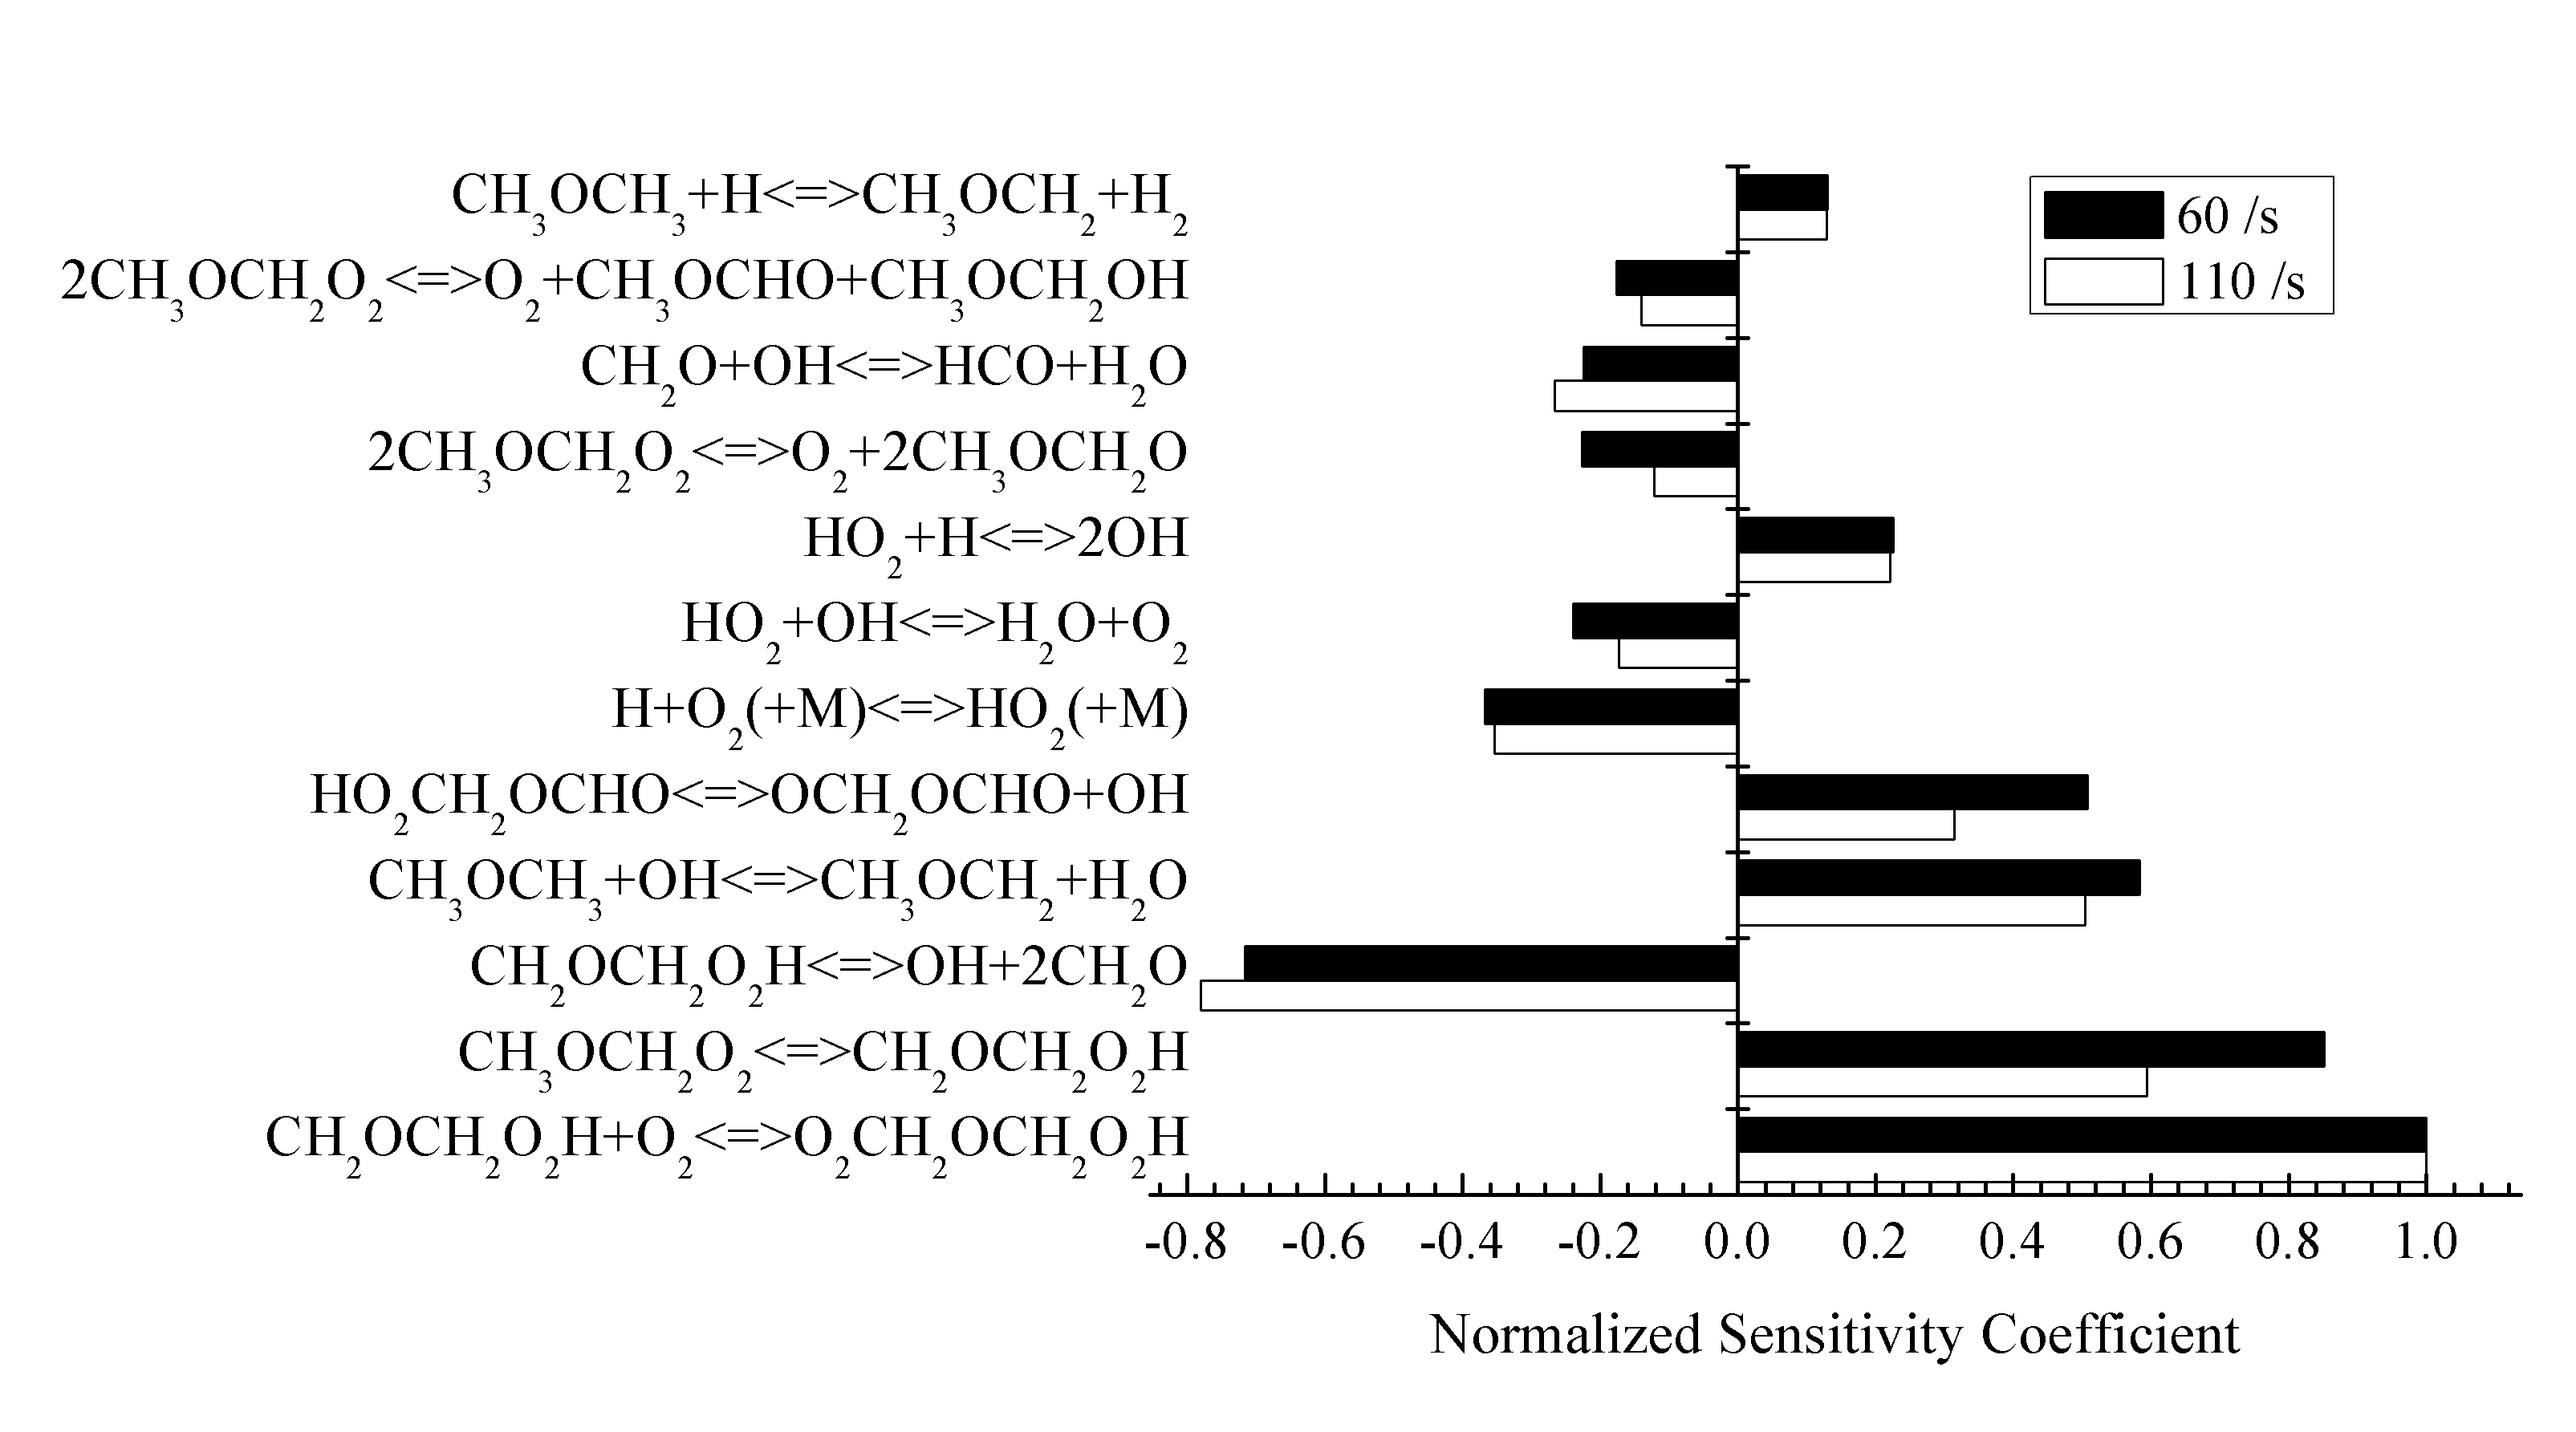
\includegraphics[width=0.7\textwidth]{Sen_SR.png}
  \normalsize
  \vspace{-0.1in}
  \caption{Sensitivity analysis on low and high strain rate cases: DME mole fraction is $30\%$.}
  \label{fig:Sen_SR}
\end{figure}

In addition to the effects of strain rate on the ignition temperature, we have also evaluated the effects of DME concentration, shown and compared with the simulation results in Fig.~\ref{fig:Ign-Con}.  The simulation result basically demonstrates the insensitive nature of the NTC-affected ignition temperature to the variation of the boundary DME concentrations over an extensive range of DME concentrations, under a fixed strain rate of $60$ /s.  The experimental results again show good agreement with the simulation results.  This effect corresponds to the insensitive nature of the equivalence ratio in the low-temperature chemistry, given the fact that the first-stage delay is insensitive to the equivalence ratio in the homogeneous autoignition process~\cite{zhao13}.  Sensitivity analysis corresponding to different boundary DME concentrations were also carried out, showing the same controlling chemistry as that of Fig.~\ref{fig:Sen_SR}.

\begin{figure}[t]
  \centering
  \scriptsize
  \vspace{-0.1in}
  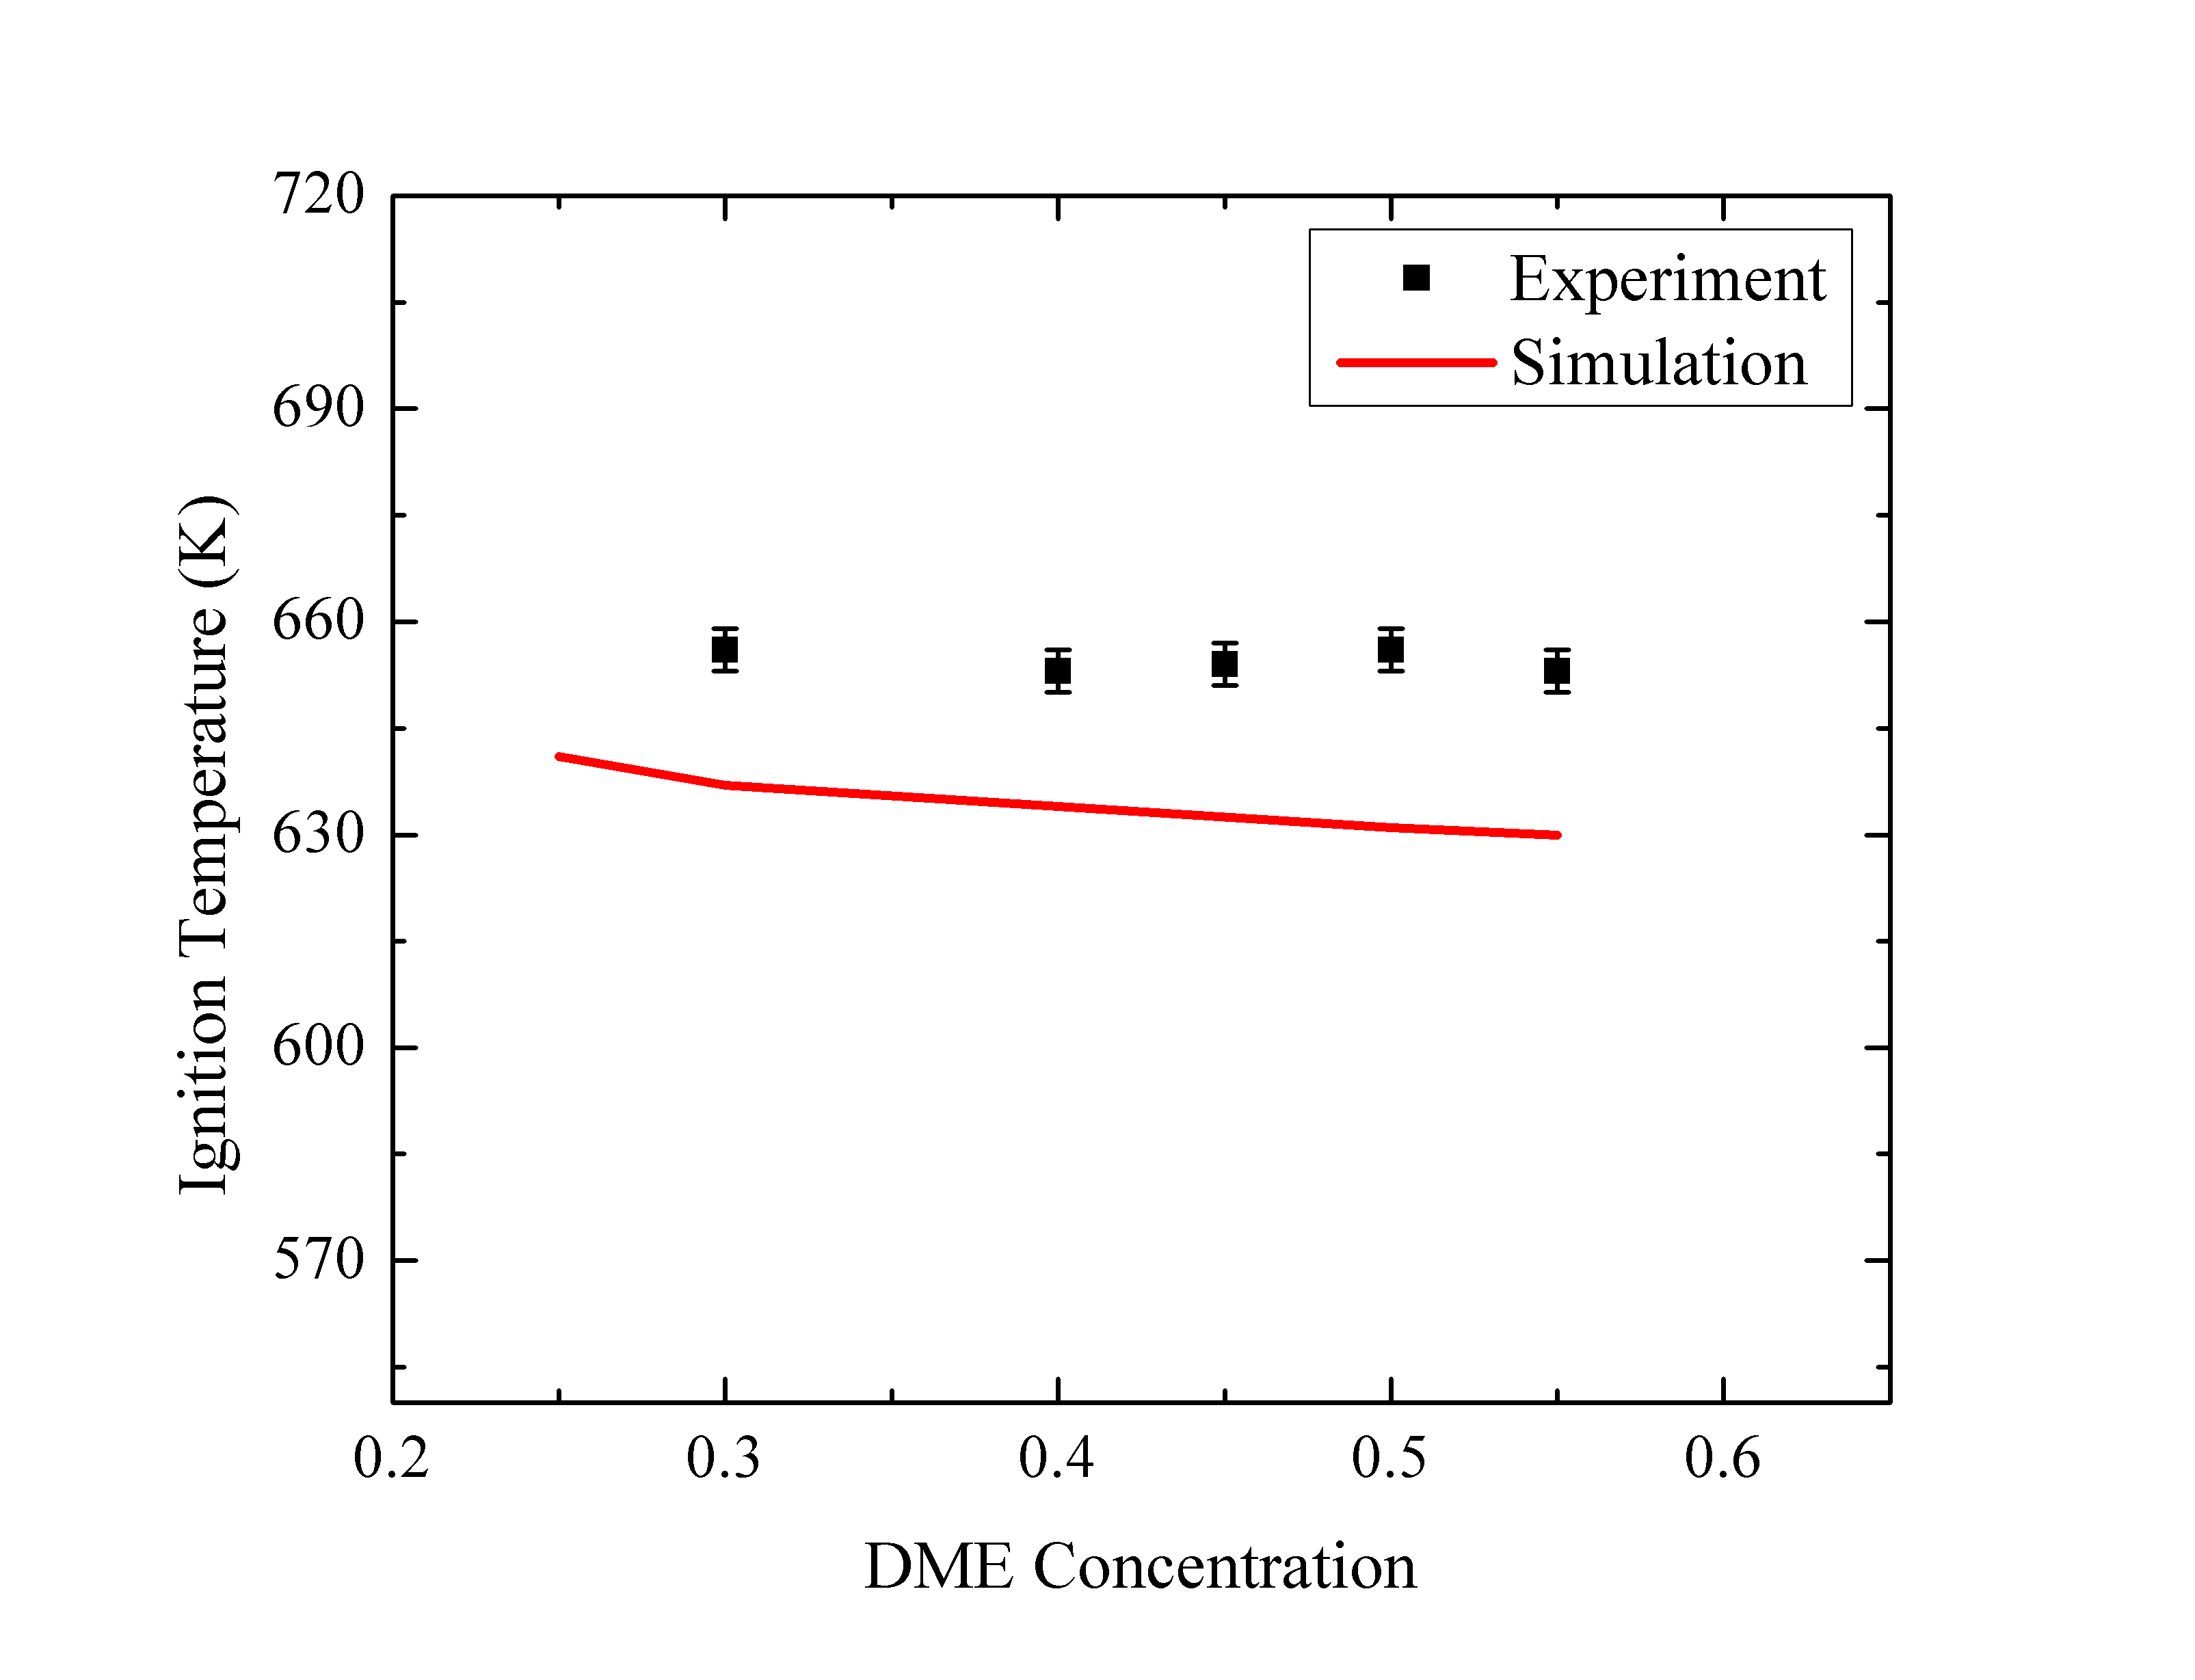
\includegraphics[width=0.6\textwidth]{Ign-Con.png}
  \normalsize
  \vspace{-0.1in}
  \caption{Ignition temperatures of various DME concentrations under the strain rate of $60$ /s.}
  \label{fig:Ign-Con}
\end{figure}


\section{Conclusions}        

Following our previous computational studies~\cite{law12,zhao13} that predicted the existence of low-temperature, NTC-affected, weakly burning diffusion flames in the counterflow, we have now successfully provided experimental substantiation of the existence of such flames.  In particular, the filtered PMT imaging demonstrated the presence of the signature HCHO chemiluminescence in the counterflow of heated air stream against nitrogen-diluted DME, while sensitive infrared imaging determined the corresponding ignition temperature.  Extensive experimentation then demonstrated that the low-temperature reactivity is enhanced with increasing air temperature, decreasing strain rate of the flow, and is insensitive to the DME concentrations.  Parallel computation substantiated the experimental results, and further corroborated the essential NTC chemistry governing the observed phenomena.

\section*{Acknowledgments}
This work was supported by the Combustion Energy Frontier Research Center, an Energy Frontier Research Center funded by the US Department of Energy, Office of Basic Energy Sciences under Award Number DE-SC0001198.

\section*{References}
\bibliographystyle{elsarticle-num-CNF}
\bibliography{NTC}

\renewcommand{\thefigure}{\arabic{figure}}
\renewcommand{\thetable}{\arabic{table}}

\end{document}


  
